%----------------------------------------------------------------------------------------
\chapter{Contribution} % possible chapter for Projects
\label{chap:contribution}

\section{Introduction to the Fair-by-Design Workflow}
\label{section:workflow-introduction}

In recent years, heightened scrutiny of the ethical implications associated with artificial intelligence (AI) and machine learning (ML) systems has arisen in response to the escalating influence of these technologies, particularly in domains where consequential decisions profoundly impact individuals' lives. The evolving landscape of AI ethics necessitates a conscientious examination of the ethical dimensions embedded in the development and deployment of these systems.

Amid this multifaceted ethical discourse, the imperative of integrating fairness into the fabric of AI design has emerged as a paramount consideration. The principle of fairness, when applied as a foundational element in the design process, underscores the need for AI systems to produce outcomes that are not only accurate and efficient but also just and equitable. Achieving fairness in AI development demands a comprehensive and deliberate approach, one that transcends mere post hoc considerations by embedding fairness principles from the very inception of the design process.

The conceptual framework of a Fair-by-Design (FBD) workflow encapsulates a meticulous set of principles and procedural steps, each strategically devised to ensure the attainment of equitable and unbiased outcomes throughout the entire lifecycle of an AI system. This includes not only the initial design and development phases but also extends to the implementation, deployment, and ongoing monitoring stages. The iterative nature of this workflow acknowledges the dynamic interplay between ethical considerations and technological advancements, emphasizing the continuous reassessment and refinement of fairness strategies.

By adopting a Fair-by-Design approach, stakeholders in AI development, ranging from researchers and engineers to policymakers and end-users, commit to a shared responsibility for cultivating a technological landscape where the ethical imperatives of fairness and equity are not afterthoughts but integral components steering the trajectory of AI systems towards societal benefit and justice. In essence, the pursuit of ethical AI underscores not only the advancement of technological capabilities but also the conscientious stewardship of these capabilities to ensure they align with ethical norms and societal values.


\subsection{Principles of Fair-by-Design Workflow}
\label{subsection:workflow-principles}

\begin{enumerate}[label=\arabic*.]
    \item \emph{Proactive Fairness Integration:}
    
    \begin{itemize}
       
        \item The cornerstone of the Fair-by-Design workflow lies in the proactive embedding of fairness considerations at the genesis of the design process, diverging from conventional practices where fairness is often retroactively addressed after system implementation.
        
        \item This proactive approach marks a transformative shift in the landscape of algorithmic development, underscoring the ethical imperative of forethought in anticipating and mitigating biases.
        
        \item Seamless integration of fairness into the initial design stages aims to forestall the emergence of discriminatory outcomes, establishing a bedrock rooted in equitable principles.
        
        \item Beyond its alignment with ethical standards, this proactive integration streamlines the developmental trajectory, fostering a more responsible and inclusive machine learning environment.
       
        \item This meticulous attention to fairness from the inception reflects a commitment to ethical AI practices that transcend mere compliance, embodying a conscientious endeavor to uphold societal values and ensure the equitable treatment of diverse individuals impacted by AI systems.
   
    \end{itemize}

    \item \emph{Transparency and Explainability:}
    
    \begin{itemize}
        
        \item The Fair-by-Design workflow places a premium on transparent documentation of design decisions and algorithmic choices, considering it a fundamental pillar of its ethical framework.
       
        \item Meticulous documentation serves as a deliberate and strategic endeavor to enhance accountability and foster trust among stakeholders.
       
        \item Each decision, ranging from the selection of specific algorithms to the fine-tuning of parameters, is comprehensively recorded, creating a clear and accessible trail of the workflow's development trajectory.
       
        \item This commitment to transparency is deeply rooted in the conviction that open communication of design rationales and choices cultivates a sense of reliability and confidence among stakeholders.
       
        \item By actively promoting transparency, the Fair-by-Design workflow contributes to the creation of a trustworthy and ethically grounded landscape for the deployment of machine learning systems.
       
        \item The deliberate and open documentation not only satisfies ethical considerations but also facilitates a more robust understanding of the system's inner workings, empowering stakeholders to engage meaningfully in the ongoing dialogue surrounding the ethical dimensions of AI technologies.
    
    \end{itemize}

    \item \emph{User-Centered Approach:}
   
    \begin{itemize}
      
        \item Within the Fair-by-Design workflow, the integration of diverse perspectives transcends a passive consideration; it stands as a proactive and integral aspect of the design process.
      
        \item The voices and perspectives of end-users and relevant stakeholders are not only actively sought but thoughtfully incorporated from the early stages of system design.
      
        \item This inclusive approach is designed to ensure that the developed system is finely tuned to the diverse needs, expectations, and concerns of its user base.
     
        \item Stakeholder engagement takes on various forms, ranging from surveys and interviews to collaborative workshops.
      
        \item These mechanisms allow for a comprehensive understanding of the social, cultural, and ethical dimensions that may influence system usage.
       
        \item Actively involving end-users and stakeholders in the design process serves a dual purpose: promoting inclusivity and enhancing the likelihood of developing a system that genuinely serves and respects the interests of its users.
       
        \item This user-centered approach is not merely a procedural step but a foundational commitment to creating AI systems that align with the values and requirements of the communities they impact.
    
    \end{itemize}

    \item \emph{Continuous Monitoring and Iterative Development:}
    
    \begin{itemize}
     
        \item Beyond the initial implementation, the Fair-by-Design system adopts a vigilant and continuous monitoring regimen, constituting a pivotal component of its iterative workflow.
     
        \item This meticulous monitoring process is crafted to detect and address emerging fairness issues that may manifest during system operation.
     
        \item Leveraging advanced monitoring tools and techniques, the workflow ensures that the system's performance is regularly assessed in real-world scenarios.
      
        \item This proactive approach enables the timely identification of potential biases or disparities, allowing for the swift implementation of corrective measures.
     
        \item The iterative nature of the workflow is a testament to its adaptability, facilitating ongoing refinements to ensure that the system evolves in response to changing dynamics and user experiences.
     
        \item This commitment to continuous monitoring and improvement underscores the Fair-by-Design philosophy: an emphasis not only on achieving fairness at a single point in time but on actively maintaining and enhancing fairness throughout the system's entire lifecycle.
      
        \item By embracing a dynamic and iterative model, the Fair-by-Design workflow remains resilient, ensuring that it remains responsive to the evolving landscape of ethical considerations and technological advancements in artificial intelligence.
   
    \end{itemize}

\end{enumerate}

\section{Steps to Implement a Fair-by-Design Workflow}
\label{section:steps}

\begin{enumerate}

    \item \emph{Objective Definition:} Clearly articulate the objectives of the system or process being designed, emphasizing the importance of fairness.

    \item \emph{Data Collection:} Determine the types of data needed for the application, establish ethical data collection protocols.

    \item \emph{Data pre-processing:} Prepare the data for the fairness algorithm, through data cleaning and featyre engineering
    
    \item \emph{Algorithmic Design and Definitions:} Define and implement fairness-enhancing algorithms across pre-processing, in-processing, and post-processing stages. Provide detailed definitions and explanations for each algorithm.

    \item \emph{Model training and evaluation:} Define the training step, performs the training tuning certain parameters and provides an evaluation of the performances of the models based on accuracy and fairness metrics.

\end{enumerate}


\begin{figure}[H]
    \centering
    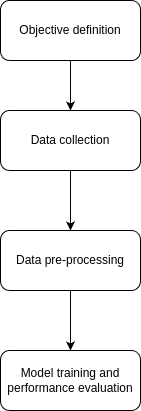
\includegraphics[width=.3\textwidth, height=.8\textwidth]{workflow-steps.png}
    \label{fig:steps}
    \caption{Fair-by-Design steps}
\end{figure}
    

\subsection{Objective Definition}
\label{subsection:objective}

The first critical step in the Fair-by-Design workflow involves a precise definition of the objectives, laying the groundwork for subsequent fairness considerations. This stage encompasses the identification of the goal of the study, the identification of protected attributes, the selection of fairness notions, and the choice of an appropriate fairness metric.

\subsubsection{Goal of the study}

The first target in the Fair-by-Design workflow is related to the identification of the goal of the whole study. It's fundamental to be able to understand whether the study requires a classification approach or a regression.


\subsubsection{Protected Attributes}

Protected attributes refer to the characteristics of individuals or groups that are explicitly considered to prevent discrimination and bias. The criteria for choosing specific protected attributes must be well-defined to ensure the relevance of fairness considerations. This may involve:

\begin{itemize}

    \item Conducting a comprehensive literature review to identify historically disadvantaged or underrepresented groups.
    
    \item Collaborating with domain experts, ethicists, and stakeholders to determine attributes with potential societal impact.
    
    \item Assessing the legal and ethical implications of including or excluding certain attributes within the specific context of the AI application.

\end{itemize}

The selected protected attributes form the basis for subsequent fairness evaluations and interventions.

\subsubsection{Fairness Notions}

Fairness notions represent the abstract principles guiding the desired equitable behavior within the AI system. The choice of fairness notions is a pivotal decision, influencing subsequent stages of the workflow. Common fairness notions, as explained in detail in \cref{section:fairness_notions}, include:

\begin{itemize}
  
    \item \textbf{Demographic Parity:} Ensuring equal representation of protected groups across different outcomes.
  
    \item \textbf{Equalized Odds:} Balancing the true positive and false positive rates across protected groups.
  
    \item \textbf{Individual Fairness:} Treating similar individuals similarly, regardless of their protected attributes.
   
    \item \textbf{Group Fairness:} Ensuring fair treatment for entire groups, typically based on statistical measures.

\end{itemize}

The selection of a fairness notion should align with the specific goals of the AI application, ethical considerations, and legal requirements.

\subsubsection{Fairness Metric}

A fairness metric quantifies the level of fairness achieved by the AI system with respect to the chosen fairness notion. The choice of a fairness metric depends on the specific fairness notion and the underlying characteristics of the data. Common fairness metrics include:

\begin{itemize}
   
    \item \textbf{Disparate Impact:} Measures the ratio of favorable outcomes between protected and unprotected groups.
   
    \item \textbf{Equalized Odds Difference:} Quantifies the disparity in error rates between protected groups.
   
    \item \textbf{Theil Index:} Evaluates the distribution of outcomes across different demographic groups.
   
    \item \textbf{Statistical Parity Difference:} Measures the difference in favorable outcomes between protected and unprotected groups.

\end{itemize}

\subsubsection{Fairness Notions and Metric Alignment}
\label{subsub:alignment}

The alignment between fairness notions and fairness metrics is a critical aspect of the Fair-by-Design workflow, as it establishes a systematic and measurable framework for evaluating fairness. The following considerations guide the selection process:

\paragraph{Demographic Parity:}

For the fairness notion of Demographic Parity, the primary concern is ensuring equal representation of protected groups across different outcomes. This notion is often aligned with the fairness metric known as \textbf{Disparate Impact}, which quantifies the ratio of favorable outcomes between protected and unprotected groups. Specifically, the Disparate Impact metric is calculated as:

\[
\text{Disparate Impact} = \frac{\text{Favorable Outcome Rate for Protected Group}}{\text{Favorable Outcome Rate for Unprotected Group}}
\]

A Disparate Impact value close to 1 indicates a balanced representation, while values significantly deviating from 1 may suggest unfairness.

\paragraph{Equalized Odds:}

The Equalized Odds fairness notion aims to balance the true positive and false positive rates across protected groups. This aligns with the \textbf{Equalized Odds Difference} fairness metric, which quantifies the disparity in error rates between protected groups. The Equalized Odds Difference is computed as:

\[
\text{Equalized Odds Difference} = \text{True Positive Rate}_{\text{Protected}} - \text{True Positive Rate}_{\text{Unprotected}}
\]

A value of 0 indicates perfect balance, with positive or negative values signifying imbalances in the error rates.

\paragraph{Individual Fairness:}

Individual Fairness focuses on treating similar individuals similarly, regardless of their protected attributes. This notion is inherently challenging to quantify, but proxy metrics such as \textbf{Theil Index} may be employed. The Theil Index evaluates the distribution of outcomes across different demographic groups and is given by:

\[
\text{Theil Index} = \sum \left( \frac{X_{i}}{\mu} \ln \frac{X_{i}}{\mu} \right)
\]

where \(X_{i}\) represents the outcome distribution for a specific group, and \(\mu\) is the overall average outcome. A lower Theil Index indicates a more equitable distribution.

\paragraph{Group Fairness:}

Group Fairness ensures fair treatment for entire groups, typically based on statistical measures. The \textbf{Statistical Parity Difference} is a common metric aligned with this notion. It measures the difference in favorable outcomes between protected and unprotected groups and is computed as:
\[
\text{Statistical Parity Difference} = \text{Favorable Outcome Rate}_{\text{Prot}} - \text{Favorable Outcome Rate}_{\text{Unprot}}
\]
A value of 0 suggests parity, while positive or negative values indicate disparities.

\begin{figure}[H]
    \centering
    \begin{tabular}{|c|c|}
        \hline
        \textbf{Fairness notion} & \textbf{Fairness metric} \\
        \hline
        Demographic Parity & Disparate Impact \\
        \hline
        Equalized Odds & Equalized Odds Difference \\
        \hline
        Individual Fairness & Theil Index \\
        \hline
        Group Fairness & Demographic Parity Difference \\
        \hline
    \end{tabular}
    \caption{Fairness metric and notion alignment}
    \label{fig:alignment}
\end{figure}

\subsubsection{Choosing Fairness Metrics Given Notions or Vice Versa}

Choosing a fairness metric given a fairness notion, or vice versa, requires a nuanced understanding of the specific fairness goals and the characteristics of the data. Here's a step-by-step guide:

\paragraph{Given a Fairness Notion:}

\begin{enumerate}
 
    \item \textbf{Define Fairness Goals:} Clearly articulate the fairness goals, considering the desired equitable outcomes for protected groups.
 
    \item \textbf{Identify Relevant Fairness Notion:} Select the fairness notion that aligns most closely with the defined fairness goals (e.g., Demographic Parity, Equalized Odds, Individual Fairness, or Group Fairness).
 
    \item \textbf{Choose Aligned Fairness Metric:} Based on the selected fairness notion, choose the fairness metric that provides a quantitative measure of the specified fairness goals (e.g., Disparate Impact, Equalized Odds Difference, Theil Index, or Statistical Parity Difference).

\end{enumerate}

\paragraph{Given a Fairness Metric:}

\begin{enumerate}

    \item \textbf{Understand Fairness Metric:} Gain a deep understanding of the chosen fairness metric, considering its strengths, limitations, and relevance to specific fairness goals.

    \item \textbf{Determine Fairness Notion Alignment:} Identify the fairness notion that aligns with the underlying principles of the chosen fairness metric (e.g., Disparate Impact aligns with Demographic Parity).
 
    \item \textbf{Ensure Consistency:} Confirm that the selected fairness metric is consistent with the broader fairness goals and ethical considerations of the AI application.

\end{enumerate}

This decisional process is well-represented in the following image:

\begin{figure}[H]
    \centering
    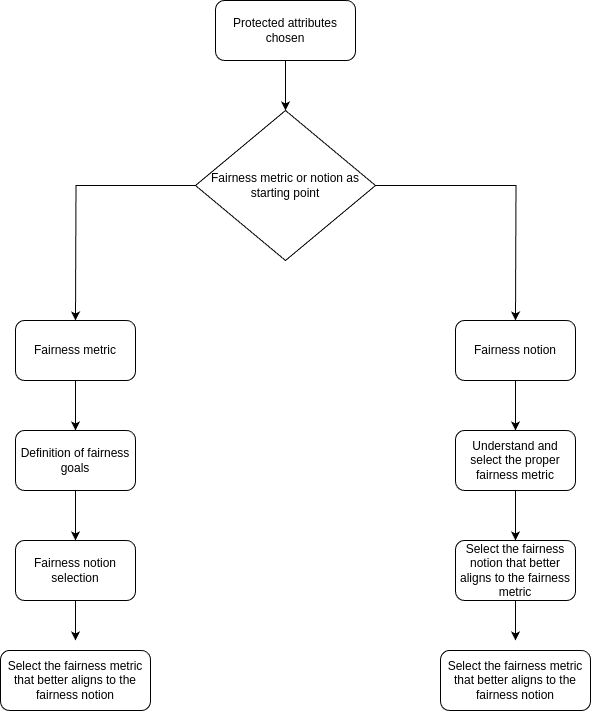
\includegraphics[width=.9\textwidth, height=1.3\textwidth]{notion-metric.png}
    \label{fig:choice}
    \caption{Fairness Notion and Metric choice}
\end{figure}

This meticulous alignment process ensures that the chosen fairness metrics quantitatively capture the intended fairness notions, providing a meaningful and interpretable basis for evaluating and comparing fairness across different models and interventions within the Fair-by-Design workflow.

In summary, the objective definition stage of the Fair-by-Design workflow involves a meticulous and well-informed selection of protected attributes, fairness notions, and fairness metrics. This precision ensures the subsequent stages of the workflow are grounded in a robust foundation for addressing bias and promoting fairness in AI systems.

\subsection{Data Collection}
\label{subsection:data_collection}

The data collection stage is fundamental for the Fair-by-Design workflow. It involves systematically gathering data to train machine learning models, coupled with a detailed study of the dataset's statistical properties, with a specific focus on protected attributes.

\subsubsection{Dataset Overview}

\paragraph{Data Representation:}
\begin{itemize}
    \item Define features and their types (categorical, numerical).
    \item Specify the structure of the data, especially in the context of demographic information.
\end{itemize}

\paragraph{Data Sources:}
\begin{itemize}
    \item Transparently describe the origin of the data (surveys, administrative records, etc.).
    \item Indicate methods used for data collection, emphasizing potential biases introduced.
\end{itemize}

\subsubsection{Study of Statistical Properties}

\paragraph{Descriptive Statistics:}
\begin{itemize}
    \item Present essential statistics: mean, median, standard deviation, quartiles (for numerical features).
    \item Provide frequency distributions (for categorical features).
\end{itemize}

\paragraph{Exploration of Protected Attributes:}
\begin{itemize}
    \item Calculate distributional metrics: proportions, counts, entropy.
    \item Focus on understanding the representation of different groups within protected attributes.
\end{itemize}

\paragraph{Correlation Analysis:}
\begin{itemize}
    \item Explore correlations between features, especially with protected attributes.
    \item Utilize correlation matrices and scatter plots for visual assessment.
\end{itemize}

\paragraph{Outlier Detection:}
\begin{itemize}
    \item Employ statistical methods or visualizations to detect and analyze outliers.
    \item Highlight the potential impact of outliers on model training and fairness considerations.
\end{itemize}

\subsubsection{Outputs for Data Pre-processing}

\paragraph{Feature Engineering Possibilities:}
\begin{itemize}
    \item Leverage insights from the dataset overview for feature engineering opportunities.
    \item Consider transformations or combinations of features to enhance model performance and fairness.
\end{itemize}

\paragraph{Bias Identification:}
\begin{itemize}
    \item Use statistical properties, especially focused on protected attributes, to identify potential biases.
    \item Understand the distribution of groups within protected attributes for addressing fairness concerns.
\end{itemize}

\paragraph{Data Cleaning Strategies:}
\begin{itemize}
    \item Formulate strategies based on outlier detection and correlation analysis.
    \item Decide on the treatment of outliers and correlations, impacting overall model quality and fairness.
\end{itemize}

\paragraph{Fairness-Aware Sampling Techniques:}
\begin{itemize}
    \item If disparities exist in the representation of different groups, consider fairness-aware sampling.
    \item Aim to address imbalances during data pre-processing for equitable model training.
\end{itemize}

In summary, the data collection stage provides the necessary foundation for the Fair-by-Design workflow. It includes a comprehensive understanding of the dataset's statistical properties and guides informed data pre-processing decisions, crucial for developing fair and unbiased machine learning models.

\subsection{Data Pre-processing}
\label{subsection:data_pre_proc}

The data pre-processing stage is a critical component of the Fair-by-Design workflow, designed to transform the raw dataset obtained from the data collection stage into a format suitable for training machine learning models. This stage involves intricate processes, including converting categorical attributes into numerical representations and handling protected attributes with specific considerations.

\subsubsection{Categorical to Numerical Transformation}

Categorical attributes, often represented as strings, must be converted into numerical format to facilitate their integration into machine learning models.

\paragraph{One-Hot Encoding:}
One-hot encoding is a widely used method for categorical attributes without a natural order. It transforms a categorical attribute with \(K\) distinct categories into \(K\) binary columns, each indicating the presence or absence of a specific category. This approach prevents the model from assigning unintended ordinal relationships to the categories.

\paragraph{Ordinal Encoding:}
When there exists an ordinal relationship between categories, ordinal encoding is applied. In this method, each category is assigned a numerical value based on its order. This preserves the ordinal information while representing the categorical attribute in a numerical format.

\paragraph{Label Encoding:}
For binary categorical attributes, label encoding is employed. It assigns 0 and 1 to the respective categories, providing a straightforward numerical representation that aligns with the binary nature of the attribute.

\subsubsection{Protected Attribute Transformation}

Protected attributes, which play a pivotal role in ensuring fairness, require special treatment during the data pre-processing stage.

\paragraph{Discrete Protected Attributes:}
If a protected attribute is discrete (e.g., gender, ethnicity), it is left unchanged during the transformation process. This ensures that the inherent categories of the attribute are preserved, and the model can account for these categories without introducing bias.

\paragraph{Continuous Protected Attributes: Quantization Operation}
Continuous protected attributes, such as age, undergo a quantization process. Quantization is a method to discretize the continuous attribute into equal-width bins. This operation is represented mathematically as:

\[ Q(x) = \text{{floor}}\left(\frac{{x - \text{{min}}}}{{\text{{bin width}}}}\right) \]

where \( Q(x) \) denotes the quantized value of \( x \), \(\text{{min}}\) is the minimum value of the attribute, and the bin width is determined based on insights from the data collection stage. The goal is to create discrete bins that accurately represent the distribution of the continuous attribute within the population. This process ensures fairness by preserving the underlying characteristics of the attribute while converting it into a suitable format for machine learning models.

Quantization is particularly essential for continuous protected attributes to avoid introducing bias during the transformation. It aligns with the overarching goal of the Fair-by-Design workflow to maintain fairness throughout the machine learning model development.

In summary, the data pre-processing stage involves sophisticated transformations, ensuring that both categorical attributes are numerically represented and protected attributes are handled with precision. These steps are crucial for developing fair and accurate machine learning models within the Fair-by-Design framework.

\subsection{Algorithm design}
\label{subsection:algorithm}

he stage of Algorithm Design within the fair-by-design workflow stands as a pivotal phase wherein the selection, adaptation, or creation of machine learning models takes place to harmonize with the specified objectives and fairness considerations. The primary objective is to craft models that not only excel in accuracy but also steadfastly adhere to ethical and fair principles. This section undertakes an in-depth exploration of the crucial considerations, strategic approaches, and the step-by-step implementation processes entailed in Algorithm Design. By navigating through these aspects, the aim is to foster the development of models that not only deliver superior performance but also champion the ideals of ethics and fairness in their predictive outcomes.

\subsubsection{Key Considerations}

\begin{enumerate}

    \item \emph{Fairness-Aware Model Selection:} 
    
    The selection of machine learning models assumes a pivotal role in the pursuit of fairness objectives. Fairness-aware model selection entails the deliberate consideration of models equipped with inherent mechanisms to tackle biases and advocate for equitable outcomes. Noteworthy examples of such models include adversarial networks, fairness-aware classifiers, and re-weighted learning algorithms. These models are systematically explored and evaluated for their capacity to mitigate biases and foster fairness, thereby contributing to the overarching goal of cultivating just and impartial predictive systems.
    
    \item \emph{Regularization Techniques:} 
    
    In the pursuit of fair predictions, regularization methods, exemplified by demographic parity constraints or equalized odds constraints, emerge as instrumental tools. These methodologies are strategically employed to guide machine learning models towards fairness objectives. By integrating fairness constraints into the optimization process, these regularization techniques play a pivotal role in steering the model to yield equitable outcomes across various demographic groups. The inclusion of such constraints serves as a proactive measure to counteract biases and ensure that the predictive power of the model remains impartial and just across diverse demographic contexts.

    \item \emph{Bias Detection and Mitigation:} 
    
    The integration of embedding mechanisms within the algorithm to detect and mitigate biases is of paramount importance. This entails the ongoing and systematic monitoring of the model's predictions for any indications of disparate impact. Subsequently, corrective measures are implemented in real-time to mitigate biases as they manifest. This proactive approach to bias detection and mitigation serves as a fundamental component in ensuring the model's fairness and equity. By embedding mechanisms that facilitate continuous scrutiny and timely interventions, the algorithm is fortified to deliver more impartial and just predictions, aligning with the principles of ethical and fair machine learning.

    \item \emph{Pre-processing, In-processing, or Post-processing Algorithms:} 
    
    The strategic decision regarding the selection of pre-processing, in-processing, or post-processing algorithms is intricately tied to the specific characteristics of the data and the defined fairness goals. Pre-processing algorithms, characterized by their ability to transform the dataset prior to model training, set the initial conditions for fairness considerations. In-processing algorithms, on the other hand, directly modify the learning process during model training, introducing fairness mechanisms at this crucial stage. Post-processing algorithms, as the name implies, come into play after model training, adjusting predictions to align with fairness objectives.

    When making this strategic decision, it is imperative to consider the nature of biases inherent in the data, the characteristics of the available dataset, and the desired level of fairness. Each approach—pre-processing, in-processing, or post-processing—offers distinct advantages and considerations, and the choice among them should be informed by a comprehensive understanding of the specific fairness challenges and objectives inherent to the machine learning task at hand.

\end{enumerate}

\subsubsection{Strategic choice for the fairness algorithm}

The strategic decision regarding the adoption of pre-processing, in-processing, or post-processing algorithms is a nuanced and crucial aspect of the Fair-by-Design workflow. This decision is intricately tied to the specific characteristics of the data and the defined fairness goals, and it plays a pivotal role in shaping the overall fairness of the machine learning model.

\textbf{Pre-processing Algorithms}

Pre-processing algorithms, distinguished by their capacity to transform the dataset before model training, establish the initial conditions for fairness considerations. This phase is especially significant in mitigating biases present in the raw data. Pre-processing techniques aim to preprocess data to make it more amenable to fairness considerations during subsequent stages. The choice of pre-processing algorithms is closely tied to the fairness goals defined for the machine learning task.

\paragraph{Relation to Fairness Goals:}
The selection of pre-processing algorithms should align with the fairness goals established at the outset of the workflow. For example, if the goal is to ensure equal representation of different demographic groups, pre-processing algorithms may focus on re-sampling or re-weighting strategies to balance the distribution of protected attributes.

\paragraph{Dependency on Fairness Notion:}
The choice between pre-processing, in-processing, or post-processing is heavily influenced by the fairness notion chosen. If the goal is to achieve demographic parity, pre-processing algorithms may involve adjusting the composition of the dataset to ensure proportional representation.

\paragraph{Evaluation Metrics:}
Metrics used to evaluate the effectiveness of pre-processing algorithms include statistical parity, disparate impact, or equal opportunity. The selection of the metric is contingent on the fairness goals and the specific aspects of fairness being prioritized.

\textbf{In-processing Algorithms}

In-processing algorithms intervene directly during the model training process, introducing fairness mechanisms at this crucial stage. This approach modifies the learning process to ensure fairness considerations are embedded in the model's development.

\paragraph{Relation to Fairness Goals:}
In-processing algorithms should be tailored to the specific fairness goals defined for the task. For instance, if the objective is to minimize disparate impact, in-processing techniques may involve adjusting the model's objective function to incorporate fairness constraints.

\paragraph{Dependency on Fairness Notion:}
The choice of in-processing algorithms depends on the fairness notion guiding the workflow. If the focus is on individual fairness, algorithms may be designed to treat similar individuals similarly during the learning process.

\paragraph{Evaluation Metrics:}
Metrics such as equalized odds, calibration, or predictive parity are often employed to assess the fairness of in-processing algorithms. The selection of the metric aligns with the fairness goals and the particular aspects of fairness under consideration.

\textbf{Post-processing Algorithms}

Post-processing algorithms come into play after model training, adjusting predictions to align with fairness objectives. This approach offers a corrective mechanism to fine-tune model outputs based on fairness considerations.

\paragraph{Relation to Fairness Goals:}
Post-processing algorithms should be chosen to complement the defined fairness goals. If the aim is to rectify disparate impact in predictions, post-processing techniques may involve re-calibrating predicted probabilities.

\paragraph{Dependency on Fairness Notion:}
The choice of post-processing algorithms is contingent on the fairness notion guiding the workflow. If the focus is on group fairness, post-processing methods may involve re-weighting predictions to achieve parity across protected attribute groups.

\paragraph{Evaluation Metrics:}
Common evaluation metrics for post-processing algorithms include reweighted accuracy, demographic parity, or predictive rate parity. The choice of the metric is aligned with the specific fairness goals and considerations.

\textbf{Strategic Decision Factors}

When making the strategic decision among pre-processing, in-processing, or post-processing algorithms, several factors come into play:

\paragraph{Nature of Biases:}
Understanding the nature of biases inherent in the data is crucial. Pre-processing algorithms may be more suitable for mitigating biases present in the raw dataset, while in-processing or post-processing algorithms may address biases emerging during model training or predictions.

\paragraph{Characteristics of the Dataset:}
The characteristics of the available dataset, such as its size, composition, and distribution of protected attributes, influence the choice of algorithmic approaches. Pre-processing may be favored for large-scale dataset adjustments, while in-processing or post-processing may be more suitable for fine-tuning models with specific biases.

\paragraph{Desired Level of Fairness:}
The desired level of fairness, whether it is absolute parity or a more nuanced balance, guides the strategic decision. Pre-processing, in-processing, or post-processing may be chosen based on the granularity required to achieve the defined fairness goals.

In essence, the choice among pre-processing, in-processing, or post-processing algorithms should be informed by a comprehensive understanding of the specific fairness challenges and objectives inherent to the machine learning task at hand. The alignment with the chosen fairness notion and the careful consideration of evaluation metrics ensure that the selected algorithmic approach is well-suited to achieve the desired fairness outcomes within the Fair-by-Design workflow.

\subsubsection{Detailed Implementation Steps}

% Include the detailed implementation steps for each key consideration as per the previous discussion.

\textbf{Fairness-Aware Model Selection}

\begin{itemize}

    \item \emph{Exploration of Fairness-Aware Models:}
     
    \begin{itemize}
    
        \item In the endeavor to develop a fair-by-design machine learning model, a pivotal step involves conducting an exhaustive survey and evaluation of existing fairness-aware models tailored to the specific application domain. This meticulous process requires a thorough examination of pertinent literature and available models, taking into account their performance metrics, interpretability, and fairness considerations. By subjecting existing models to rigorous evaluation, practitioners gain valuable insights into the nuanced strengths and limitations of different approaches. This discerning survey and evaluation process empower practitioners to make informed decisions regarding the most suitable model for their particular use case. Such diligence contributes significantly to the foundational aspects of a fair-by-design workflow, ensuring that the selected model not only aligns with technical requirements but also upholds ethical considerations inherent to the application domain.
    
        \item When delving into the realm of fairness-aware models tailored for a specific application domain, it is judicious to prioritize models explicitly designed to address bias. This consideration encompasses, but is not confined to, adversarial networks or models featuring inherent fairness constraints. Adversarial networks serve the purpose of mitigating bias by introducing a secondary network that identifies and counteracts any discriminatory patterns discerned in the primary model. Conversely, models with built-in fairness constraints integrate predefined fairness metrics into the optimization process, ensuring the model adheres to fairness criteria throughout training.

        The evaluation of these specialized models yields a nuanced understanding of their efficacy in handling bias, furnishing practitioners with invaluable insights into the most suitable approach for mitigating bias within their specific context. This deliberate consideration solidifies the fair-by-design approach, underscoring the paramount importance of selecting models that actively address and rectify biases to foster equitable outcomes in the realm of machine learning applications.    
    
    \end{itemize}
    
    \item \emph{Implementation and Customization:}
    
    \begin{itemize}
    
        \item Following the selection of a fairness-aware model tailored for the specific application domain, the subsequent imperative involves its implementation within the chosen machine learning framework. This intricate process necessitates the translation of model specifications and architecture into code, meticulous configuration of essential parameters, and seamless integration into the overarching machine learning pipeline. The implementation procedure should strictly adhere to industry best practices and guidelines stipulated by the chosen framework, ensuring not only optimal performance but also seamless compatibility.

        Furthermore, developers must prioritize the interpretability of the model, recognizing that transparency is pivotal in comprehending how fairness considerations are intricately embedded within the system. The successful execution of the implementation phase represents a pivotal juncture in the fair-by-design workflow. It sets the groundwork for subsequent stages encompassing model training, rigorous evaluation, and eventual deployment, all underscored by an unwavering commitment to fostering equitable and unbiased machine learning outcomes.    
    
        \item Subsequent to the implementation of the chosen fairness-aware model, a pivotal phase entails customizing the model to harmonize with the unique characteristics of the dataset and the precise fairness objectives delineated earlier in the workflow. This customization process necessitates the fine-tuning of model parameters, adjustment of hyperparameters, and incorporation of features that aptly accommodate the nuanced intricacies present in the dataset.

        Moreover, developers may find it imperative to introduce specific fairness-oriented adjustments to the model's architecture. This ensures the model's adeptness in effectively handling and mitigating biases associated with protected attributes. Such meticulous and tailored customization stands as an indispensable step for optimizing the model's performance within the paradigm of the fair-by-design approach. Here, the overarching objective extends beyond technical excellence, encompassing the ethical imperative of delivering unbiased machine learning outcomes.    
    
    \end{itemize}

\end{itemize}

\textbf{Explainability and Interpretability}

\begin{itemize}

    \item \emph{Model Selection:}

    \begin{itemize}

        \item Within the fair-by-design workflow, the strategic choice of models renowned for their high explainability and interpretability holds paramount significance. Decision trees and rule-based models, celebrated for their inherent transparency, stand out as preferred choices in this context. The rationale underpinning this selection is deeply rooted in the commitment to transparency and accountability.

        Models characterized by easy interpretability empower stakeholders, including end-users and decision-makers, to comprehend the intricate decision-making processes. This transparency not only cultivates trust but also facilitates the identification and mitigation of any potential biases or fairness concerns embedded within the model. By deliberately opting for models with high explainability, the fair-by-design workflow aligns seamlessly with its overarching goal of cultivating machine learning systems that excel not only in technical robustness but also in ethical soundness, ensuring they are readily understandable by a diverse range of stakeholders.

        \item Within the fair-by-design workflow, when infusing fairness considerations into model selection, a critical aspect is to judiciously navigate the trade-offs between model complexity and interpretability. The optimal balance hinges significantly on the specific application requirements, playing a pivotal role in the decision-making process.

        Highly complex models, while potentially offering superior predictive performance, often come at the cost of diminished interpretability. Conversely, interpretable models such as decision trees or rule-based models may exhibit limitations in capturing intricate patterns present in the data. Striking the right balance becomes paramount; the fair-by-design approach is not solely concerned with ensuring fairness but also places a premium on transparency.
        
        Therefore, the strategic selection of models aligning with the interpretability needs of stakeholders while still meeting performance requirements becomes a key consideration in the design process. This deliberate and conscious decision-making process contributes significantly to the development of machine learning models that are not only fair but also understandable and accountable, embodying the principles of the fair-by-design approach.

    \end{itemize}

\end{itemize}

\textbf{Regularization Techniques}

\begin{itemize}

    \item \emph{Integration of Fairness Constraints:}

    \begin{itemize}

        \item The incorporation of fairness constraints mandates a nuanced comprehension of the precise fairness goals and metrics germane to the application domain. In the fair-by-design approach, there is a pronounced emphasis on the principled and systematic integration of these constraints into the machine learning model's training process. This deliberate embedding of fairness into the training regimen aims to mitigate biases and advocate for equitable outcomes.

        The overarching objective of the fair-by-design workflow extends beyond the mere delivery of accurate predictions. It is intricately woven with the commitment to ethical and fairness considerations, thereby contributing substantively to the cultivation of responsible and unbiased machine learning practices. This concerted effort reinforces the imperative of aligning machine learning models with ethical principles, ensuring they operate within a framework that prioritizes fairness and equity.

        \item Within the fair-by-design approach to machine learning, a pivotal facet involves the systematic experimentation with various regularization techniques. These methods, exemplified by demographic parity constraints or equalized odds constraints, assume a substantial role in the concerted effort to mitigate biases and champion fairness within machine learning models. Tailored to address specific fairness considerations linked to protected attributes, these techniques are meticulously designed to ascertain that the model's predictions remain uninfluenced by factors such as gender, race, or other sensitive attributes. This intentional and exploratory engagement with regularization techniques underscores the commitment to cultivating models that not only excel in predictive accuracy but also uphold the ethical imperative of fairness and equity.
    
    \end{itemize}

\end{itemize}

\textbf{Bias Detection and Mitigation}

\begin{itemize}
    
    \item \emph{Dynamic Bias Mitigation:}
    
    \begin{itemize}
    
        \item A proactive strategy within the fair-by-design framework involves the development of adaptive algorithms that dynamically adjust to emerging biases in the data. These algorithms are meticulously designed to engage in continuous monitoring and evaluation of the model's performance, adept at identifying any potential biases that may manifest during operational phases. The adaptive nature of these algorithms empowers them to dynamically tweak parameters or decision boundaries in response to emerging biases, thereby ensuring an ongoing commitment to fairness in real-world applications. This forward-thinking approach aligns seamlessly with the ethos of the fair-by-design framework, emphasizing not only initial fairness but also the continuous vigilance and adaptation necessary for sustained equity in machine learning outcomes.

        \item A pivotal step in the fair-by-design workflow involves the implementation of corrective measures, such as re-weighting or re-sampling, to actively mitigate biases as they are detected. As biases are identified through ongoing monitoring, these targeted corrective measures are strategically applied to address imbalances and promote fairness in the model's predictions. This iterative and adaptive approach not only acknowledges the inevitability of biases but also proactively works towards rectifying them, reinforcing the commitment to fairness and equity embedded within the fair-by-design methodology.

    \end{itemize}

\end{itemize}

\textbf{Human-in-the-Loop Approaches}

\begin{itemize}
    
    \item \emph{Stakeholder Collaboration:}
    
    \begin{itemize}
    
        \item Organize collaborative sessions with domain experts and stakeholders to delve into the intricacies of fairness considerations. These sessions serve as a platform for a comprehensive exploration of nuances related to fairness, leveraging the collective insights and expertise of domain specialists and key stakeholders. The aim is to foster a shared understanding of fairness challenges, identify contextual nuances, and coalesce diverse perspectives. Such collaborative endeavors contribute significantly to the fair-by-design approach, ensuring that the developed models align not only with technical requirements but also with the ethical and contextual considerations of the specific application domain.
    
        
        \item Engage stakeholders actively in both model validation and decision-making processes. This participatory approach ensures that the perspectives and insights of stakeholders are integral to the validation of the model's performance and the decision-making procedures. By involving stakeholders, including end-users and decision-makers, in these crucial stages, the fair-by-design workflow embraces transparency and inclusivity. This collaborative involvement contributes to the development of models that are not only technically sound but also align with the diverse needs and expectations of the stakeholders, fostering a sense of ownership and accountability in the overall machine learning process.
    
    \end{itemize}

\end{itemize}

\subsubsection{Pre-processing Algorithm Proposed}

\paragraph{Fairness through data augmentation}
\label{subsec:ftdr}

IIn this approach, the paradigm of bias mitigation takes on a unique and innovative perspective, one that prioritizes data augmentation over attribute removal. Unlike traditional approaches that center on the exclusion of specific attributes, this methodology embraces the concept of data augmentation, introducing a distinctive definition of fairness and equity within the AI system.

The essence of this approach revolves around the augmentation of the dataset by introducing new data instances that offer a more comprehensive and inclusive representation of the underlying population. This expanded dataset is designed to be more diverse, representative, and balanced, transcending the limitations of the original data and fostering a more nuanced understanding of fairness. 

The introduction of augmented data instances leads to a redefined notion of fairness within the AI system. Instead of solely focusing on the absence of biased attributes, fairness is now measured in terms of the dataset's inclusivity and its ability to capture the diversity and nuances present within the population it seeks to serve. 

This approach aligns with the broader philosophy of ensuring that AI systems are equitable, just, and capable of making informed and unbiased decisions. By augmenting the dataset, it strives to bridge the gaps in representation and provide a more equitable playing field for all individuals, regardless of their background or characteristics. 

The process of data augmentation necessitates a careful selection of techniques and methodologies that can introduce new data instances while maintaining the integrity and quality of the dataset. These techniques may encompass oversampling, synthetic data generation, or other data synthesis methods, each tailored to the specific context and objectives of the AI system.

In traditional fairness definitions, the focus often revolves around ensuring fair treatment for individual protected attributes, denoted as $A_1, A_2, \ldots, A_k$. While this is undoubtedly crucial, a more comprehensive understanding of fairness calls for an examination of fairness in the context of combinations of protected attributes and the output. A new definition of fairness is proposed, which takes into account the representation of all combinations of $k$ protected attributes and the output, aiming for equitable representation across these combinations.

A fair dataset is defined as one in which, for each combination of protected attributes $\{A_1, A_2, \ldots, A_k\}$ and the output $O_j$, the representation is equal and proportional. Mathematically, a dataset is fair if:

\[
\forall i_1, i_2, \ldots, i_k, j: \frac{|D_{i_1, i_2, \ldots, i_k, j}|}{|D|} = \text{constant}
\]

where:
\begin{itemize}

    \item $D$ is the dataset

    \item $|D_{i_1, i_2, \ldots, i_k, j}|$ is the number of samples with the specific combination of protected attributes $A_{i_1}, A_{i_2}, \ldots, A_{i_k}$ and output $O_j$

    \item $|D|$ is the total number of samples in the dataset
    
\end{itemize}

This entails that any combination of demographic groups, defined by the protected attributes, and the output should have comparable representation, thereby fostering a balanced and unbiased dataset.

By striving for equal representation of combinations of protected attributes, is addressed a fundamental aspect of fairness that transcends individual attributes. This approach provides a more nuanced understanding of fairness by considering the intersections of various demographic groups. It encourages a broader examination of potential biases that may arise when considering multiple attributes simultaneously.

Incorporating this definition of fairness into the data augmentation process enables us to promote a comprehensive notion of fairness, aligning with the principles of equal opportunity and non-discrimination across all combinations of protected attributes. The subsequent algorithm and experimental evaluation are designed to actualize this definition and demonstrate its effectiveness in achieving a more equitable representation within the dataset.

Let $D$ be a dataset $R^{n \times m}$, where $n$ is the number of samples and $m$ is the number of features. Let $k$ be the number of protected variables represented as $R^{n \times 1}$, with $u_i$ the number of unique values for the $i$-th protected variable. Let there be a single output variable represented as $R^{n \times 1}$.

A data augmentation function $\mathcal{R}$ can be formally defined as a mapping:
\[
\mathcal{R}: R^{n \times m} \rightarrow R^{a \times m}
\]
where $a > n$, and the function $\mathcal{R}$ transforms the input dataset $D$ of dimensions $n \times m$ into an output dataset $D'$ of dimensions $a \times m$.

The number of possible combinations of these variables is $\prod_{i=1}^{k+1} u_i$. The limit of the product is ${k + 1}$ because for the combination are considered the protected attributes together with the output.

Consider a set $\text{Combinations}$ with occurrences of all $\prod_{i=1}^{k+1} u_i$ combinations within the dataset. 

Consider a set $\text{Frequencies}$ with frequency of all combination in $\text{Combinations}$ set.

For each combination, the number of rows in which that combination appears should be equal to the maximum of $\text{Frequencies}$ set, denoted as $\text{Max(Frequencies)}$

Mathematically, the number of rows ($a - n$) that will be added to the dataset by the data augmentation algorithm is given by:
\[
a - n = \sum_{i=1}^{|Combinations|}(\text{Max}(\text{Frequency}) - (\text{Frequency\textunderscore i}))
\]

Once having detected the number of rows to add for each combination it's important to define how to are detected the element of each row.

Let $C$ be the sub-dataset of $D$ with a specific combination $\text{c\textunderscore i}$ for the protected attributes. Given the number of rows \text{Max}(\text{Frequency}) - (\text{Frequency\textunderscore i}) each row is added according to the following rules:

\begin{itemize}
    
    \item The values of the protected and output variables are set according to the specific combination.
   
    \item For all other attributes, a random value $\text{random\_value}_{ij}$ is generated, where $j$ represents the specific attribute, and $i$ represents the row being added for that attribute. $\text{random\_value}_{ij}$ is within the minimum and maximum range for attribute $j$.

\end{itemize}

Before proceeding in the theoretical analysis of the algorithm here's the proposed pseudocode:

\begin{algorithm}[H]
    \caption{Reabalancing}
    \begin{algorithmic}[1]
        \State \textbf{Input:} combination\_set, combination\_frequency, protected\_attributes, dataset\_attributes
        \State \textbf{Output:} Updated dataset

        \State max\_frequency $\gets$ max(combination\_frequency)

        \For{index \textbf{in} (0, len(combination\_set) - 1)}
            \State combination $\gets$ combination\_set[index]
            \State frequency $\gets$ combination\_frequency[index]
            \State combination\_dataset $\gets$ dataset[dataset[combination] == combination\_set[index]]

            \While{frequency $<$ max\_frequency}
                \State new\_row $\gets$ empty

                \For{(attr, val) \textbf{in} (combination, protected\_attributes)}
                    \State new\_row[attr] $\gets$ val
                \EndFor

                \For{attr \textbf{in} dataset\_attributes \textbf{and not in} protected\_attributes}
                    \State new\_row[attr] $\gets$ random(min(combination\_dataset[attr]), max(combination\_dataset[attr]))
                \EndFor

                \State dataset.add(new\_row)
                \State frequency $+$= 1
            \EndWhile
        \EndFor

        \State \textbf{return} Updated dataset
    \end{algorithmic}
\end{algorithm}

The proposed data augmentation algorithm aims to achieve fairness by ensuring an equal representation of all possible combinations of protected and output variables. Here, we provide a theoretical analysis of the algorithm's key aspects, including time complexity, space complexity, and additional considerations.

The time complexity is influenced by the dataset size ($n$), the number of features ($m$), and the number of combinations of protected attributes and output. The overall time complexity is given by the number of combinations:
\[
\mathcal{O}(n \cdot m \cdot |Combinations|)
\]
where $|Combinations|$ is the number of combinations that have been computed

The space complexity is determined by the storage of combination frequencies and the occurrence count array. The overall space complexity is given by:
\[
\mathcal{O}(\prod_{i=1}^{k+1} u_i)
\]

\begin{itemize}
    \item \textbf{Number of Combinations:} The number of combinations \(\prod_{i=1}^{k+1} u_i\) grows exponentially with the number of protected binary variables (\(k\)), significantly influencing both time and space complexity.
    
    \item \textbf{Data Augmentation Techniques:} The algorithm's effectiveness depends on the chosen data augmentation techniques, which may introduce additional computational costs.
    
    \item \textbf{Random Value Generation:} The quality of randomness in generated values is crucial for the diversity of the augmented dataset and, consequently, the algorithm's fairness outcomes.
    
    \item \textbf{Implementation and Optimization:} The efficiency of the algorithm is affected by implementation details, language choice, and potential optimizations.
\end{itemize}

\subsubsection{Significance}

The Algorithm Design stage is pivotal in shaping the ethical and fair behavior of machine learning models within the fair-by-design framework. By carefully selecting, customizing, and integrating fairness-aware models, and incorporating transparency and human-in-the-loop approaches, this stage ensures that the resulting models align with ethical considerations and promote equitable outcomes.

\subsection{Model training and evaluation}
\label{subsection:model-training}

\subsubsection{Introduction}

This section delivers a thorough overview of the model training and evaluation process within the Fair-by-Design framework. After the careful application of the chosen pre-processing, in-processing, or post-processing algorithm, the training phase assumes a pivotal role in shaping a machine learning model. The emphasis extends beyond mere accuracy objectives to incorporate the ethical considerations of fairness. This holistic approach underscores the commitment to developing models that excel not only in predictive performance but also adhere to principles of equity and justice, thereby embodying the ethos of the Fair-by-Design framework.

\subsubsection{Training Process}

\paragraph{Data Splitting}

The dataset undergoes a deliberate split into training, validation, and test sets, each serving a distinct strategic purpose. The training set acts as the foundation for the model's learning process, enabling it to grasp patterns and relationships within the data. The validation set plays a crucial role in hyperparameter tuning, fine-tuning the model to enhance its generalization capabilities. Finally, the test set serves as the litmus test for the final model's performance, offering a reliable measure of its predictive capabilities. This meticulous division ensures a comprehensive and robust evaluation of the model's effectiveness and generalizability within the Fair-by-Design framework.

\paragraph{Model Architecture}

The architecture of the selected model is meticulously crafted to strike a delicate balance between accuracy and fairness considerations within the Fair-by-Design framework. Architectures may incorporate innovative components, such as adversarial layers or customized modules specifically designed to enforce fairness constraints. The focal point is to develop a model that excels not only in capturing intricate patterns but is also interpretable and transparent in its decision-making process. This intentional design reflects the commitment to fostering models that go beyond predictive prowess, embodying principles of interpretability and transparency while addressing fairness concerns.

\paragraph{Training Parameters}

Critical training parameters, spanning the learning rate, batch size, and convergence criteria, undergo meticulous tuning in the Fair-by-Design framework. The learning rate assumes significance as it dictates the step size in the optimization process, thereby influencing the pace of updates to model parameters. This parameter is pivotal in determining the balance between the model's adaptability and stability during training.

The batch size, another key parameter, determines the number of samples processed in each iteration. This factor significantly impacts the overall efficiency of the training process, influencing resource utilization and the model's ability to generalize well to diverse datasets.

Convergence criteria hold a crucial role by ensuring that the training process halts when the model achieves optimal performance. These criteria are indispensable in preventing overfitting, safeguarding against the model becoming excessively tailored to the training data to the detriment of its ability to generalize to new, unseen data.

This comprehensive tuning process, applicable beyond deep models, reflects a nuanced approach in optimizing key parameters to foster models that not only exhibit accuracy but also align with fairness considerations in the Fair-by-Design paradigm.

\paragraph{Fairness Constraints}

In scenarios where fairness constraints are seamlessly integrated into the training process within the Fair-by-Design framework, a deliberate and systematic approach is adopted. These constraints are explicitly defined and enforced, often involving the introduction of regularization terms designed to penalize disparate treatment of different demographic groups. This strategic incorporation aims to instill fairness by discouraging the model from exhibiting biased behavior towards specific groups.

Adversarial training components might also be leveraged in this process. These components act as a countermeasure to mitigate bias, introducing a dynamic element that works to identify and neutralize any discriminatory patterns that may emerge during training. The overall objective is to foster models that not only deliver accurate predictions but also adhere to ethical principles of fairness and equity. This intentional integration of fairness constraints reinforces the commitment to cultivating machine learning models that contribute to just and unbiased outcomes.

\paragraph{Model Training}

The model undergoes training for a specified number of iterations, leveraging the training set to iteratively update its parameters and increase accuracy. This iterative training process is not limited to deep learning models and is applicable across various model categories. The overarching goal remains to strike a balance between accuracy and fairness, contributing to the development of a machine learning model proficient in capturing underlying patterns while being conscious of potential biases.

Through successive iterations on the training set, the model refines its understanding of the data, aiming to optimize its performance with due consideration to fairness. This approach aligns with the principles of the Fair-by-Design framework, ensuring that the trained model is both technically robust and ethically sound in its decision-making, irrespective of the specific model category employed.

\subsubsection{Evaluation Metrics}

\paragraph{Accuracy Metrics}

A suite of accuracy metrics is employed to holistically assess the model's overall performance:

\begin{itemize}
    \item \emph{Accuracy:} The ratio of correctly predicted instances to the total instances.
    
    \item \emph{Precision:} The proportion of true positive predictions among instances predicted as positive.
    
    \item \emph{Recall:} The proportion of true positive predictions among actual positive instances.
    
    \item \emph{F1-score:} The harmonic mean of precision and recall, providing a balanced measure of accuracy.
\end{itemize}

\paragraph{Fairness Metrics}

Fairness metrics are instrumental in evaluating the model's behavior across different demographic groups:

\begin{itemize}
    
    \item \emph{Equalized Odds Evaluation Metric}: The Equalized Odds metric serves as a critical assessment tool for gauging the model's performance concerning fairness. This evaluation metric specifically investigates whether the model exhibits comparable false positive and false negative rates across distinct demographic groups. By scrutinizing disparities in these rates, the Equalized Odds metric offers insights into the model's capacity to provide equitable outcomes for diverse segments of the population, contributing to a comprehensive understanding of its fairness considerations, as reported in \cref{section:metrics}
    
    \item \emph{Statistical Parity:} The Statistical Parity metric is a meticulous examination of the distribution of positive outcomes within each demographic group. This evaluation metric meticulously analyzes the proportion of positive results for each group, aiming to identify and quantify any disparities that may exist. By shedding light on these disparities, the Statistical Parity metric offers a nuanced perspective on how the model's predictions align with different demographic segments. This in-depth analysis contributes to a comprehensive assessment of fairness, facilitating a more detailed understanding of potential imbalances in positive outcomes across diverse groups, as reported in \cref{section:metrics}

\end{itemize}

\subsubsection{Results and Analysis}

\paragraph{Accuracy Results}

A meticulous analysis of accuracy results stands as a cornerstone in gaining valuable insights into the model's predictive prowess concerning the target variable. Precision, recall, and F1-score metrics play a pivotal role in offering a nuanced understanding of the intricate trade-offs between true positives, false positives, and false negatives.

Precision provides insights into the accuracy of positive predictions, recall assesses the model's ability to capture all positive instances, and the F1-score encapsulates a harmonized view, considering both precision and recall. The overarching goal transcends mere accuracy; it extends to cultivating a balanced and informed prediction capability. This multifaceted evaluation approach ensures a comprehensive grasp of the model's performance, allowing for a nuanced interpretation of its predictive accuracy while considering the intricate interplay between different performance metrics.

\paragraph{Fairness Results}

Fairness metrics serve as a crucial lens through which biases within the model are identified and addressed. Disparate impact, equalized odds, and statistical parity results undergo thorough analysis to evaluate whether the model demonstrates disparate treatment among various demographic groups. The emphasis is not only on recognizing but also on actively mitigating disparities, fostering the development of a model that upholds principles of fairness and equity. By leveraging these metrics, the evaluation process goes beyond traditional performance measures, ensuring a diligent scrutiny of how the model's predictions may impact different demographic segments and actively working towards an unbiased and equitable predictive system.

\paragraph{Trade-offs}

Comprehending the nuanced trade-offs between accuracy and fairness is pivotal in the pursuit of a balanced model. Achieving this equilibrium may necessitate adjustments to the model. Techniques such as re-weighting, re-sampling, or the introduction of customized loss functions can be employed to specifically address fairness concerns that arise during evaluation. The central theme becomes striking the right balance—ensuring optimal performance of the model while actively addressing and mitigating fairness considerations. This delicate calibration process is intrinsic to refining the model, aligning it not only with accuracy goals but also with the ethical imperative of fostering fairness and equity in its predictions.

\subsubsection{Discussion}

\paragraph{Interpretability}

The interpretability of the model's decisions holds paramount importance. Techniques such as SHAP (SHapley Additive exPlanations) values or LIME (Local Interpretable Model-agnostic Explanations) are thoroughly explored to enhance transparency in the decision-making process. The focus is on understanding and elucidating how the model arrives at its predictions. This commitment to interpretability contributes significantly to the model's trustworthiness, providing stakeholders with clear insights into the factors influencing predictions. By adopting these interpretability techniques, the model not only meets technical excellence standards but also aligns with the broader goal of fostering trust and confidence in its decision-making capabilities.

\paragraph{Ethical Considerations}

The discussion extends beyond technical aspects to encompass ethical considerations arising from the model's behavior. Rigorous attention is dedicated to uncovering potential biases, identifying unintended consequences, and evaluating the impact on different demographic groups. Strategies for addressing ethical concerns are thoughtfully proposed, emphasizing a steadfast commitment to responsible and ethical AI practices. This holistic examination ensures that the model's deployment aligns not only with technical efficacy but also with a profound awareness of its societal implications, fostering a responsible and ethical approach to artificial intelligence.

\paragraph{Further Refinement}

Derived from the observed results, proposals for further refinement are thoughtfully put forth. This iterative process may encompass adjusting fairness constraints, fine-tuning hyperparameters, or exploring alternative algorithms, all aimed at enhancing both accuracy and fairness in model predictions. The iterative nature of this refinement process underscores a steadfast commitment to continuous improvement and the unwavering pursuit of fairness. This dynamic approach ensures that the model evolves in response to insights gained from its performance, fostering a resilient and adaptive system that continually strives to achieve the highest standards of accuracy and fairness.

